\chapter{PRUEBAS Y RESULTADOS}
\label{cap:resultados}

\section{Plan de pruebas de la solución}
\label{sec:plan-pruebas}

La verificación se planificó por subsistema y por nivel de evidencia. Las pruebas son numéricas, analíticas y geométricas: análisis estructural del bastidor y de sus uniones, modelos de elementos finitos de los centradores, barridos en el modelo CAD, cálculo de la red hidráulica y simulación del mojado del rodamiento. Los ensayos físicos quedan fuera del alcance de la tesis; ningún resultado de este capítulo es una validación experimental.

Se adoptó un Caso Base por subsistema. Para el soporte, el Caso Base es el bastidor de tres apoyos sectoriales con el rodamiento centrado y una carga vertical de $3\times9948$ N. Para la aspersión, el Caso Base hidráulico fue la red de diecinueve boquillas y el Caso Base de mojado, la configuración de 22 boquillas a 1,7 rpm. A partir de ellos se plantearon escenarios de sensibilidad y de rediseño: combinaciones de carga con factores 1,00, 1,25 y 1,40; fuerza final del centrador de 1,45 a 2,08 kN; desvío lateral de una rueda; presión uniforme de 3 a 6 bar en las boquillas; cambio de malla, paso de tiempo, dominio y número de parcelas del modelo de mojado; y las variantes de boquillas del diámetro exterior y de la cara inferior. La Tabla~\ref{tab:plan-pruebas} asigna a cada prueba sus escenarios, sus variables, su criterio y su estado.

\begingroup
\small\singlespacing
\setlength{\tabcolsep}{3.5pt}
\renewcommand{\arraystretch}{1.08}
\begin{longtable}{@{}>{\raggedright\arraybackslash}p{2.9cm}>{\raggedright\arraybackslash}p{3.7cm}>{\raggedright\arraybackslash}p{3.0cm}>{\raggedright\arraybackslash}p{1.9cm}>{\raggedright\arraybackslash}p{\dimexpr\textwidth-11.5cm-10\tabcolsep\relax}@{}}
\caption{Plan de pruebas, escenarios y estado}\label{tab:plan-pruebas}\\
\toprule
\textbf{Prueba} & \textbf{Caso Base y escenarios} & \textbf{Variables medidas} & \textbf{Criterio} & \textbf{Estado}\\
\midrule\endfirsthead
\caption[]{Plan de pruebas, escenarios y estado (continuación)}\\
\toprule
\textbf{Prueba} & \textbf{Caso Base y escenarios} & \textbf{Variables medidas} & \textbf{Criterio} & \textbf{Estado}\\
\midrule\endhead
\midrule\multicolumn{5}{r}{\textit{Continúa en la página siguiente.}}\\\endfoot
\bottomrule\endlastfoot
Análisis estructural del bastidor & Carga centrada; factores 1,00, 1,25 y 1,40; desvío lateral de una rueda y tiro de las cadenas & Reacciones, flecha relativa, D/C de barras y uniones & E03, E04, E05 & Ejecutada\\
Modelo global con cargas de centrado & 1,45, 1,60 y 2,08 kN; alabeo libre, continuo o impedido en los nudos & Desplazamiento en el contacto del centrador & E06, E08 & Ejecutada\\
Elementos finitos locales de los centradores & 2,08 kN; dos mallas y dos sentidos de carga & Desplazamiento radial y tensiones & E06, E08 & Ejecutada\\
Error de colocación y captura & Fuerza final del empujador; excentricidad de 5 mm en ocho direcciones & Error de colocación y carrera de captura & E06, E08 & Ejecutada (cálculo)\\
Barridos CAD e interferencias & Traslado, giro del distribuidor, retirada de la lanza y centradores & Holgura mínima y contactos & E01, E07, E15 & Ejecutada\\
Red hidráulica & 19, 22 y 24 boquillas; presión uniforme de 3 a 6 bar & Presión por boquilla, caudal, altura, potencia, NPSH & E09--E11 & Ejecutada\\
Simulación del mojado & 22 boquillas a 1,7 rpm; malla, $\Delta t$, dominio y parcelas; caso puente & Acceso, dosis, uniformidad, zona seca, transferencia e impulso & E12, E13 & Ejecutada\\
Rediseño de boquillas & Lateral inclinada y superior desplazada; par inferior de abanico estrecho (24 boquillas) & Dosis, uniformidad, zona seca y transferencia & Regla de decisión; criterio de la zona exterior & Ejecutada\\
Alcance del lavado & Dosis requerida de 65, 183 y 305 kg\,m$^{-2}$; trazado de rayos del rodamiento armado & Tiempo hasta la dosis requerida; área visible de rodillos y pistas & E13 & Ejecutada (cálculo)\\
\end{longtable}
\endgroup

El mojado se evalúa con seis indicadores propuestos por el equipo (Tabla~\ref{tab:kpi-cfd}). Miden si el líquido llega a cada superficie, cuánto llega, con qué uniformidad y con qué cantidad de movimiento; no miden la remoción de grasa, que solo puede establecerse con ensayo.

\begin{table}[htbp]
\centering\small\singlespacing
\caption{Indicadores del modelo de mojado}
\label{tab:kpi-cfd}
\begin{tabularx}{\textwidth}{@{}lY@{}}
\toprule
\textbf{Indicador} & \textbf{Definición}\\
\midrule
Acceso geométrico & Fracción del área mojable que alcanzan los chorros, por trazado de rayos con los obstáculos del soporte\\
Dosis de mojado & Masa depositada por unidad de área y por vuelta del distribuidor, $D$, media y mínima por bandas (Sección~\ref{sec:teo-cfd})\\
Uniformidad & Coeficiente de variación de $D$ entre bandas de 10 mm (y de 2 mm, complementario)\\
Zona seca & Fracción de bandas sin impacto directo, y área con $D\geq5$ kg\,m$^{-2}$ por vuelta\\
Transferencia & Fracción del caudal de las boquillas asignadas a una superficie que llega a ella, $\eta$\\
Acción hidráulica & Impulso por unidad de área y por vuelta, $J$, y presión media de huella\\
\bottomrule
\end{tabularx}
\end{table}

\section{Análisis de los resultados de las pruebas}

\subsection{Subsistema de soporte}
\label{sec:resultados-soporte}

\subsubsection{Caso Base: análisis estructural del bastidor}

El bastidor de tres apoyos sectoriales se analizó en SAP2000 como pórtico de barras W6$\times$9 de acero ASTM A36, con las cargas del rodamiento en los nodos de los apoyos sectoriales y cuatro apoyos en las posiciones de las ruedas \cite{csi_analisis_2016}. Los apoyos son bilaterales: el nodo 2 restringe los tres desplazamientos y los nodos 5, 13 y 16 restringen los desplazamientos en $X$ y $Z$; las rotaciones quedan libres. La Figura~\ref{fig:modelo-r01} muestra el modelo y la Tabla~\ref{tab:combinaciones-r01}, las combinaciones.

\begin{figure}[htbp]
\centering
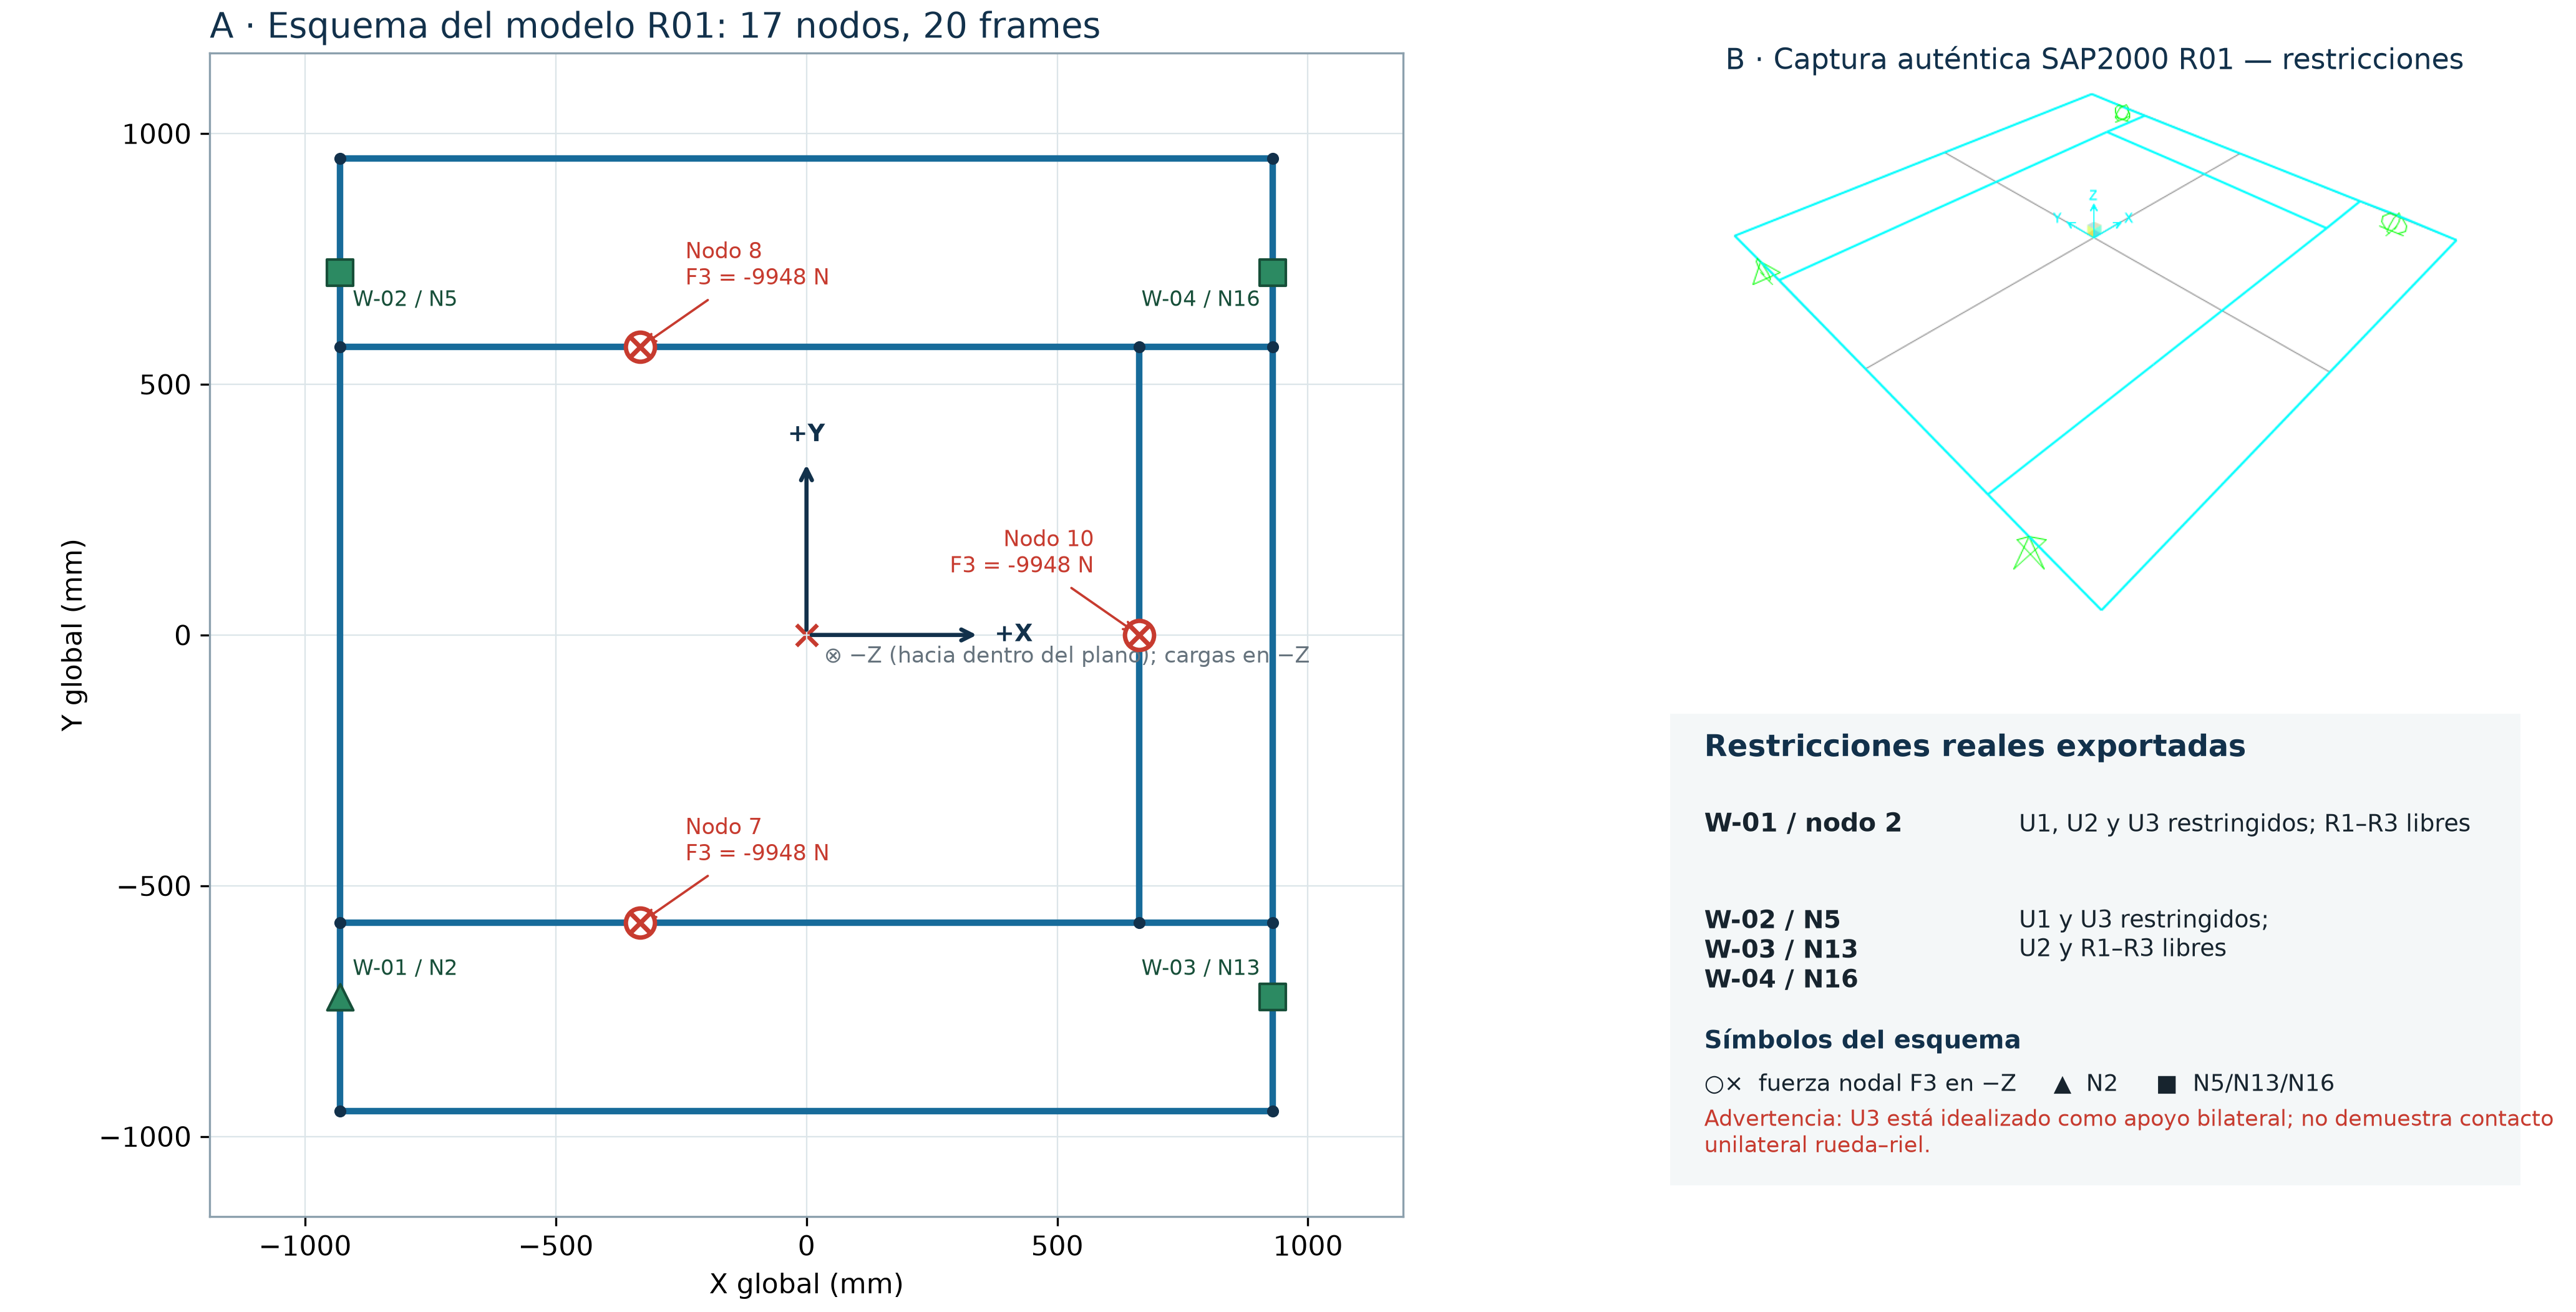
\includegraphics[width=0.84\textwidth]{images/sap/02_MODELO_CARGAS_APOYOS_R01_recorte.png}
\caption{Modelo estructural del bastidor de tres apoyos sectoriales: esquema de nodos, cargas y apoyos (izquierda) y restricciones en SAP2000 (derecha). Los apoyos verticales son bilaterales y no representan el contacto unilateral rueda--riel. Fuente: corrida del modelo en SAP2000 y posproceso propio.}
\label{fig:modelo-r01}
\end{figure}

\begin{table}[htbp]
\centering\small\singlespacing
\caption{Combinaciones de carga del análisis estructural}
\label{tab:combinaciones-r01}
\begin{tabularx}{\textwidth}{YP{3.2cm}P{3.6cm}}
\toprule
\textbf{Combinación} & \textbf{Peso propio del bastidor} & \textbf{Carga vertical en los apoyos} \\
\midrule
Nominal de servicio & 1,00 & 1,00 \\
Servicio con carga externa amplificada & 1,00 & 1,25 \\
Resistente & 1,40 & 1,40 \\
\bottomrule
\end{tabularx}
\end{table}

La combinación nominal sumó 29,844 kN de carga externa y 1,649 kN de peso propio, con una reacción total de 31,493 kN (Tabla~\ref{tab:reacciones-r01}). El cálculo manual del Anexo~\ref{anx:calculos} reprodujo las reacciones con diferencias no mayores que 0,004 N, lo que comprueba el equilibrio y el reparto del caso centrado. En la combinación resistente, la reacción total exportada fue de 44,090 kN, igual a $1{,}4(29{,}844+1{,}649)$ kN dentro de la precisión tabulada.

\begin{table}[htbp]
\centering\small\singlespacing
\caption{Reacciones verticales y resultados de servicio del bastidor}
\label{tab:reacciones-r01}
\begin{tabularx}{\textwidth}{@{}Yrr@{}}
\toprule
\textbf{Magnitud} & \textbf{Nominal de servicio} & \textbf{Carga externa $\times1{,}25$} \\
\midrule
Reacción en los nodos 2 y 5 / 13 y 16 (kN) & 7,846 / 7,900 & -- \\
Reacción individual máxima (kN) & 7,900 & 9,766 \\
Suma de reacciones verticales (kN) & 31,493 & 38,954 \\
Máximo nodal $|U_3|$ (mm) & 1,353 & 1,686 \\
Flecha relativa en el nodo del apoyo (mm) & 1,236 & 1,540 \\
Diferencia vertical entre apoyos (mm) & 0,294 & 0,367 \\
\bottomrule
\end{tabularx}
\end{table}
\label{tab:resultados-servicio}

El máximo nodal $|U_3|$ no es la flecha del miembro: para el travesaño de carga se evaluó el nodo del apoyo respecto de la cuerda de sus extremos con la Ecuación~\eqref{eq:mt-flecha}. Con la longitud del travesaño de 1860 mm, la flecha relativa nominal de 1,236 mm queda por debajo de $L/360=5{,}17$ mm, $L/800=2{,}33$ mm y $L/1000=1{,}86$ mm. Es una evaluación nodal; falta buscar el máximo continuo entre estaciones. La verificación de miembros con AISC 360-16 dio una razón demanda/capacidad máxima de 0,277 en los travesaños de carga, con la combinación resistente (Anexo~\ref{anx:programas}). Se compararon también bastidores de cuatro y cinco apoyos; el de tres tuvo la menor masa, 168,1 kg, con una flecha dentro de los límites, y se mantuvo (Anexo~\ref{anx:iteraciones}).

Ese modelo solo tenía cargas verticales. Al agregar el desvío lateral de una rueda durante el traslado, con 6,51 kN en el contacto, las vigas longitudinales pasaron de 0,28 a 0,82, y a 0,89 con el alabeo libre en los nudos (Tabla~\ref{tab:uniones-bastidor}). Las diez uniones a momento quedaron en D/C $\leq0{,}58$. El bastidor cumple, pero el margen que daba el caso vertical era engañoso: lo gobierna una carga del traslado que el primer modelo no tenía.

\subsubsection{Verificación global con las cargas de centrado}

Las cargas de los centradores son horizontales y excéntricas respecto del alma, de modo que torsionan los travesaños de carga. Con la torsión uniforme de Saint-Venant que emplea SAP2000 en sus barras, el desplazamiento en el contacto de una referencia resultó de 13 a 17 mm, un valor sin sentido físico porque ignora la rigidez al alabeo de la sección. Por ello se construyó un modelo global con siete grados de libertad por nudo, que incluye la torsión no uniforme \cite{aiscdg9}. Antes se replicó el pórtico en CalculiX: dos voladizos de calibración coincidieron con la solución analítica dentro del 2\,\% y el equilibrio cerró con residuos inferiores a $10^{-7}$ N.

Sumando la parte global y la local, el desplazamiento total en el contacto de la referencia resultó de 1,51 a 1,64 mm con uniones rígidas. Si los encuentros de los travesaños se resolvieran solo por el alma, subiría a 2,1--7,1 mm. Un travesaño adicional lo reducía a 0,77--0,78 mm, pero quedaba a 5,3--7,7 mm bajo el pie giratorio de la lanza y se retiró. El resultado llevó a diseñar las uniones a momento con continuidad de alas (Sección~\ref{sec:uniones-bastidor}) y a juzgar la deformación por su efecto sobre la colocación del rodamiento.

\subsubsection{Centradores y precisión del centrado}

Las referencias, con 0,48 a 0,59 mm en el contacto, cumplen el criterio local de 1,0 mm, aunque no siempre el objetivo de 0,5 mm. En el empujador, la placa de 20 mm del soporte del pivote presentó de 190 a 246 MPa de membrana más flexión, por encima del filtro de 150 MPa. Con una placa de 28 mm, la tensión bajó a 102--129 MPa y el desplazamiento de 1,58--1,65 a 0,89--0,91 mm; esa placa se adoptó, con soldaduras a tope de penetración completa.

En el modelo CAD, con el aro desplazado 5 mm en ocho direcciones, el rodillo de cada centrador tocó siempre antes que la horquilla, el pasador o el brazo, y la carrera de captura en el peor caso fue de 13,1 mm, frente a 5 mm de E08. La precisión era el punto débil de la segunda entrega: 5,21 mm en el caso nominal y 6,10 mm en la envolvente de 2,08 kN. Al separar la parte elástica de las tolerancias (Sección~\ref{sec:error-colocacion}), se vio que el 70\,\% del error a 2,08 kN es deformación y que crece con la fuerza. Con el ajuste H7/g6 y el límite de 1,95 kN al empujador, el error queda en 4,09 mm en la detención y 4,24 mm en el disparo, con alabeo libre, y en 3,35 mm con las alas continuas del detalle de uniones. La envolvente de 2,08 kN, que exige fallar la detención y el disparo, da 5,18 mm con alabeo libre y 3,91 mm con alas continuas.

\subsection{Subsistema de aspersión}
\label{sec:resultados-aspersion}

\subsubsection{Red hidráulica}

Al pasar de diecinueve a veintidós boquillas, el caudal aumentó un 16,4\,\% y la altura de bombeo un 3,6\,\%, y la boquilla más desfavorable pasó de una superior a la más alta de la lanza. Con 24 boquillas, el caudal subió otro 9,1\,\% y la altura 0,83 m (Tabla~\ref{tab:red-hidraulica}). Las presiones de las boquillas quedaron entre 4,00 y 4,13 bar, de modo que la red entrega un caudal casi uniforme. Entre 3 y 6 bar de presión uniforme, el caudal de la red de 22 boquillas pasa de 173,7 a 245,7 L/min y la escala de fuerza del chorro se duplica (Anexo~\ref{anx:calculos}). Más presión eleva la acción del chorro a costa de caudal y de energía, y su efecto sobre la limpieza solo puede comprobarse con ensayo.

\subsubsection{Modelo de mojado y verificación numérica}

El mojado se simuló en ANSYS Fluent con fase discreta lagrangiana acoplada en dos vías, aire con turbulencia $k$--$\varepsilon$ y paredes que retienen la gota en el primer impacto \cite{fluent2026}. El distribuidor se representó detenido en sectores de $\pm12^\circ$ alrededor de cada boquilla y la dosis por vuelta se obtuvo integrando la huella sobre la circunferencia (Sección~\ref{sec:teo-cfd}). Los obstáculos del soporte se aplicaron como máscaras de sombra por trazado de rayos. Una corrida con un apoyo sectorial incluido en la malla respaldó el método: a ese apoyo llegó el 16,9\,\% del caudal de la boquilla inferior exterior, frente al 18,0\,\% estimado con las máscaras. La configuración completa se detalla en el Anexo~\ref{anx:programas}.

La verificación de la configuración base comparó tres niveles de malla por dominio, con razones de refinamiento de 1,25 a 1,30, y estimó la incertidumbre de discretización con el índice de convergencia de malla \cite{celik2008}. Los cambios entre las dos mallas más finas y los de los demás estudios están en la Tabla~\ref{tab:verificacion-cfd} del Anexo~\ref{anx:programas}.

Los indicadores integrales cambiaron menos que el 5\,\% fijado como criterio de trabajo, y la mayoría menos del 1\,\%. En la cara inferior, los cambios quedaron dentro del ruido entre corridas equivalentes de los dos brazos ($\pm1{,}5$\,\% en $\bar D$), por lo que el índice de convergencia no es interpretable allí. La dosis mínima varió hasta $\pm18$\,\%, porque la fija una sola banda; se informa, pero no se usa para juzgar la convergencia. Con menos parcelas por boquilla aparecían zonas secas artificiales, lo que justificó usar 600 trayectorias por plano en las boquillas de incidencia normal y 1200 en las inferiores. El caso del agujero repetido en Fluent difirió del resuelto en OpenFOAM un 0,27\,\% en la dosis media; esa concordancia entre programas no equivale a una validación física.

\subsubsection{Resultados de la configuración base}

La Tabla~\ref{tab:cfd-caso-base} reúne los indicadores de la configuración base, con los obstáculos del soporte, y la Figura~\ref{fig:cfd-trayectorias} muestra las trayectorias de las gotas en el diámetro exterior y la cara inferior.

\begin{table}[htbp]
\centering\small\singlespacing
\setlength{\tabcolsep}{4pt}
\caption{Indicadores de la configuración base de 22 boquillas por superficie}
\label{tab:cfd-caso-base}
\begin{tabular}{lcccccc}
\toprule
\textbf{Superficie} & \textbf{\makecell{Acceso\\(\%)}} & \textbf{$\bar D$; $D_{mín}$} & \textbf{CV} & \textbf{Seca 10/2 mm (\%)} & \textbf{$\eta$ (\%)} & \textbf{$\bar J$}\\
\midrule
Diámetro exterior & 100 & 26,40; 0,44 & 0,302 & 0 / 0,39 & 94,3 & 609\\
Cara superior & 100 & 22,53; 6,13 & 0,396 & 0 / 0 & 97,9 & 527\\
Cara inferior & 100 & 5,46; 2,93 & 0,616 & 0 / 0 & 31,0 & 43\\
Agujero & 100 & 18,72; 11,52 & 0,339 & 0 / 0 & 86,9 & 438\\
\bottomrule
\end{tabular}
\par\smallskip\footnotesize
$D$ en kg\,m$^{-2}$ por vuelta y $J$ en N\,s\,m$^{-2}$ por vuelta, a 1,7 rpm. Acceso sobre el área mojable, que excluye las huellas de los apoyos sectoriales y la franja de los topes.
\end{table}

\begin{figure}[htbp]
\centering
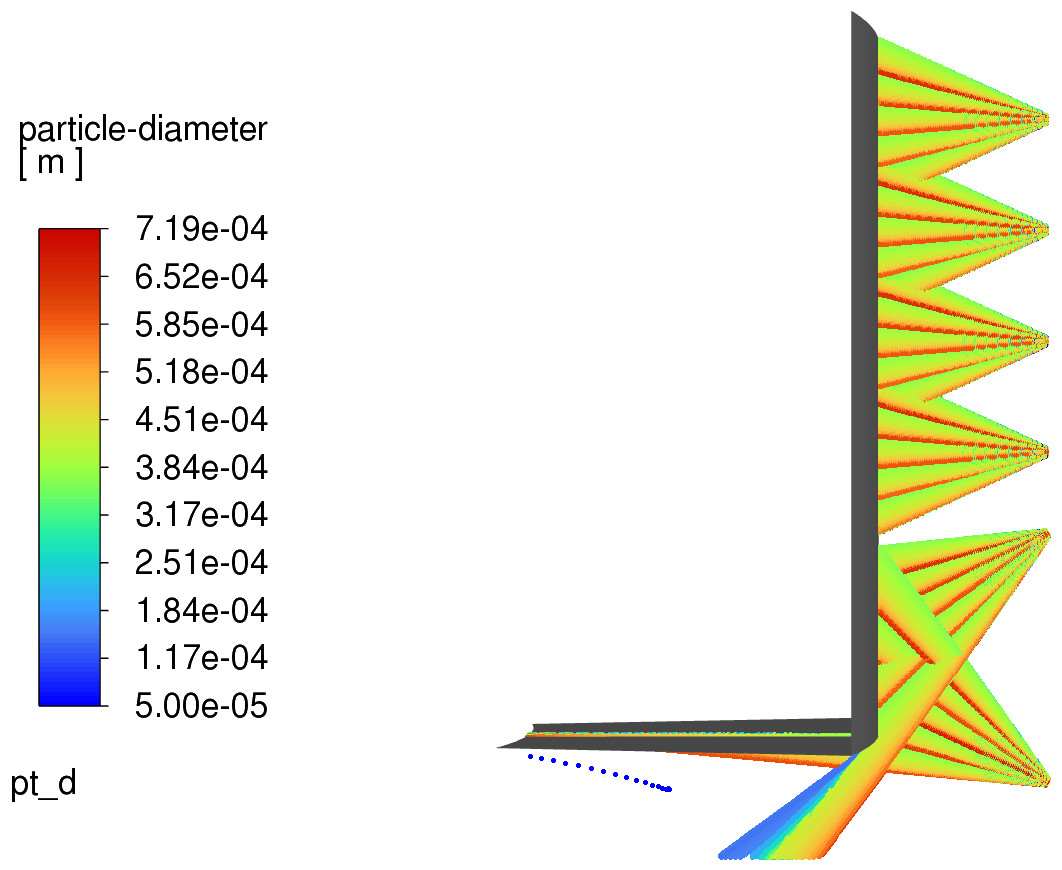
\includegraphics[width=0.62\textwidth]{fluent_gotas_od_cara_inferior.png}
\caption{Trayectorias de las gotas de las boquillas laterales e inferior exterior de un brazo sobre el diámetro exterior y la cara inferior, vista lateral, configuración base. La escala de color es el diámetro de la gota en metros (rótulo del programa en inglés). Imagen cualitativa: muestra la forma de los abanicos, no la dosis. Elaboración propia, simulación en ANSYS Fluent 2026 R1 (licencia Student); imagen recortada al área de interés.}
\label{fig:cfd-trayectorias}
\end{figure}

Ninguna superficie presentó zona seca con bandas de 10 mm. Con bandas de 2 mm, el diámetro exterior tuvo una franja de 0,39\,\% sin impacto directo entre $Z\approx1032$ y 1038 mm: el aire arrastrado por el chorro lateral más bajo desviaba hacia abajo las gotas de la boquilla inferior exterior. El acceso geométrico de las cuatro superficies fue de 99,13\,\% del área de referencia de 5,64 m$^2$; los 0,049 m$^2$ restantes son las huellas supuestas de los apoyos sectoriales (0,042 m$^2$) y la franja de los topes (0,007 m$^2$), que se asignan a la segunda etapa de lavado. Del caudal total de 202,59 L/min, el 52,1\,\% llegó al diámetro exterior, el 23,5\,\% al agujero, el 17,8\,\% a la cara superior, el 4,7\,\% a la cara inferior y el 2,0\,\% escapó.

La cara inferior es la superficie crítica. Recibió unas cuatro veces menos dosis que las demás, con la menor uniformidad y una transferencia del 31\,\%. Las gotas llegaban casi rasantes, con velocidades normales de 4,4 y 9,7 m/s frente a unos 23 m/s en las otras superficies, y su impulso era de diez a catorce veces menor. Ese resultado llevó a rediseñar las boquillas inferiores.

\subsubsection{Rediseño del diámetro exterior}

Para cerrar la franja del diámetro exterior se evaluaron dos variantes con el mismo caudal y el mismo número de boquillas. La primera inclina $-4^\circ$ la primera boquilla lateral de cada brazo; la segunda añade un desplazamiento de 15 mm hacia fuera de la segunda boquilla superior. La comparación se hizo frente a la configuración base con el brazo A duplicado, cuya franja seca de 2 mm es de 1,17\,\% (Tabla~\ref{tab:rediseno-od}).

\begin{table}[htbp]
\centering\small\singlespacing
\caption{Variantes de las boquillas del diámetro exterior y de la cara superior}
\label{tab:rediseno-od}
\begin{tabularx}{\textwidth}{@{}Yccc@{}}
\toprule
\textbf{Superficie e indicador} & \textbf{Base emparejada} & \textbf{Lateral inclinada} & \textbf{Más superior desplazada}\\
\midrule
Diámetro exterior: zona seca, bandas de 2 mm (\%) & 1,17 & 0 & 0\\
Diámetro exterior: CV, bandas de 10 mm & 0,304 & 0,265 & 0,265\\
Diámetro exterior: $D_{mín}$, bandas de 10 mm & 0,27 & 14,6 & 14,6\\
Cara superior: CV, bandas de 10 mm & 0,396 & 0,396 & 0,321\\
Cara superior: $D_{mín}$, bandas de 10 mm & 6,13 & 6,13 & 14,0\\
Cara superior: $\eta$ (\%) & 97,9 & 97,9 & 94,8\\
\bottomrule
\end{tabularx}
\par\smallskip\footnotesize
$D$ en kg\,m$^{-2}$ por vuelta. Ninguna de las dos variantes cambió la cara inferior.
\end{table}

La inclinación de la boquilla lateral basta para cerrar la franja y elevar la dosis mínima del diámetro exterior de 0,27 a 14,6 kg\,m$^{-2}$ por vuelta, sin costo de caudal; por eso se incorporó al diseño. El desplazamiento de la boquilla superior mejora además la cara superior, pero baja su transferencia en 3,1 puntos y no se incorporó al modelo CAD; queda como mejora evaluada.

\subsubsection{Configuración inferior propuesta}

La configuración de la Sección~\ref{sec:configuracion-inferior}, con 24 boquillas y la boquilla lateral inclinada, se simuló con los dos brazos explícitos, en la misma malla y con el mismo modelo que la configuración base. Las demás superficies conservaron sus resultados, porque la presión de sus boquillas cambió menos de 10 mbar. La Tabla~\ref{tab:cfd-propuesta} y la Figura~\ref{fig:cfd-propuesta} resumen los resultados.

\begin{table}[htbp]
\centering\small\singlespacing
\caption{Resultados del CFD de la configuración propuesta frente a la configuración base}
\label{tab:cfd-propuesta}
\begin{tabularx}{\textwidth}{@{}Yrrl@{}}
\toprule
\textbf{Indicador (dosis en kg\,m$^{-2}$ por vuelta)} & \textbf{Base*} & \textbf{Propuesta} & \textbf{Cambio}\\
\midrule
Cara inferior: dosis media & 5,46 & 14,16 & $\times2{,}6$\\
Cara inferior: coeficiente de variación & 0,626 & 0,430 & mejora\\
Cara inferior: dosis mínima, banda de 10 mm & 2,83 & 7,33 & $\times2{,}6$\\
Cara inferior: transferencia (\%) & 30,9 & 48,2 & $+17$ puntos\\
Zona exterior de la cara (Z3): dosis media & 4,1 & 19,99 & criterio 15,8\\
Zona exterior de la cara (Z3): coeficiente de variación & 0,246 & 0,298 & criterio $\leq0{,}4$\\
Diámetro exterior: dosis media & 26,38 & 25,82 & $-2{,}1$\,\%\\
Diámetro exterior: zona seca, bandas de 2 mm (\%) & 1,17 & 0 & se cierra\\
Cara inferior: tiempo de lavado con 183 kg\,m$^{-2}$, peor banda de 10 mm & 36,7 min & 14,7 min & 2,5 veces menos\\
\bottomrule
\end{tabularx}
\par\smallskip\footnotesize
*Base emparejada, con el brazo A duplicado; el tiempo base usa la dosis mínima de la Tabla~\ref{tab:cfd-caso-base} (2,93). Z3 es la zona de la cara inferior del aro exterior, entre los radios de 617,5 y 710 mm. El tiempo de lavado supone una dosis requerida de 183 kg\,m$^{-2}$ y 1,7 rpm, ambas hipótesis.
\end{table}

\begin{figure}[htbp]
\centering
\begin{minipage}[t]{0.49\textwidth}\centering
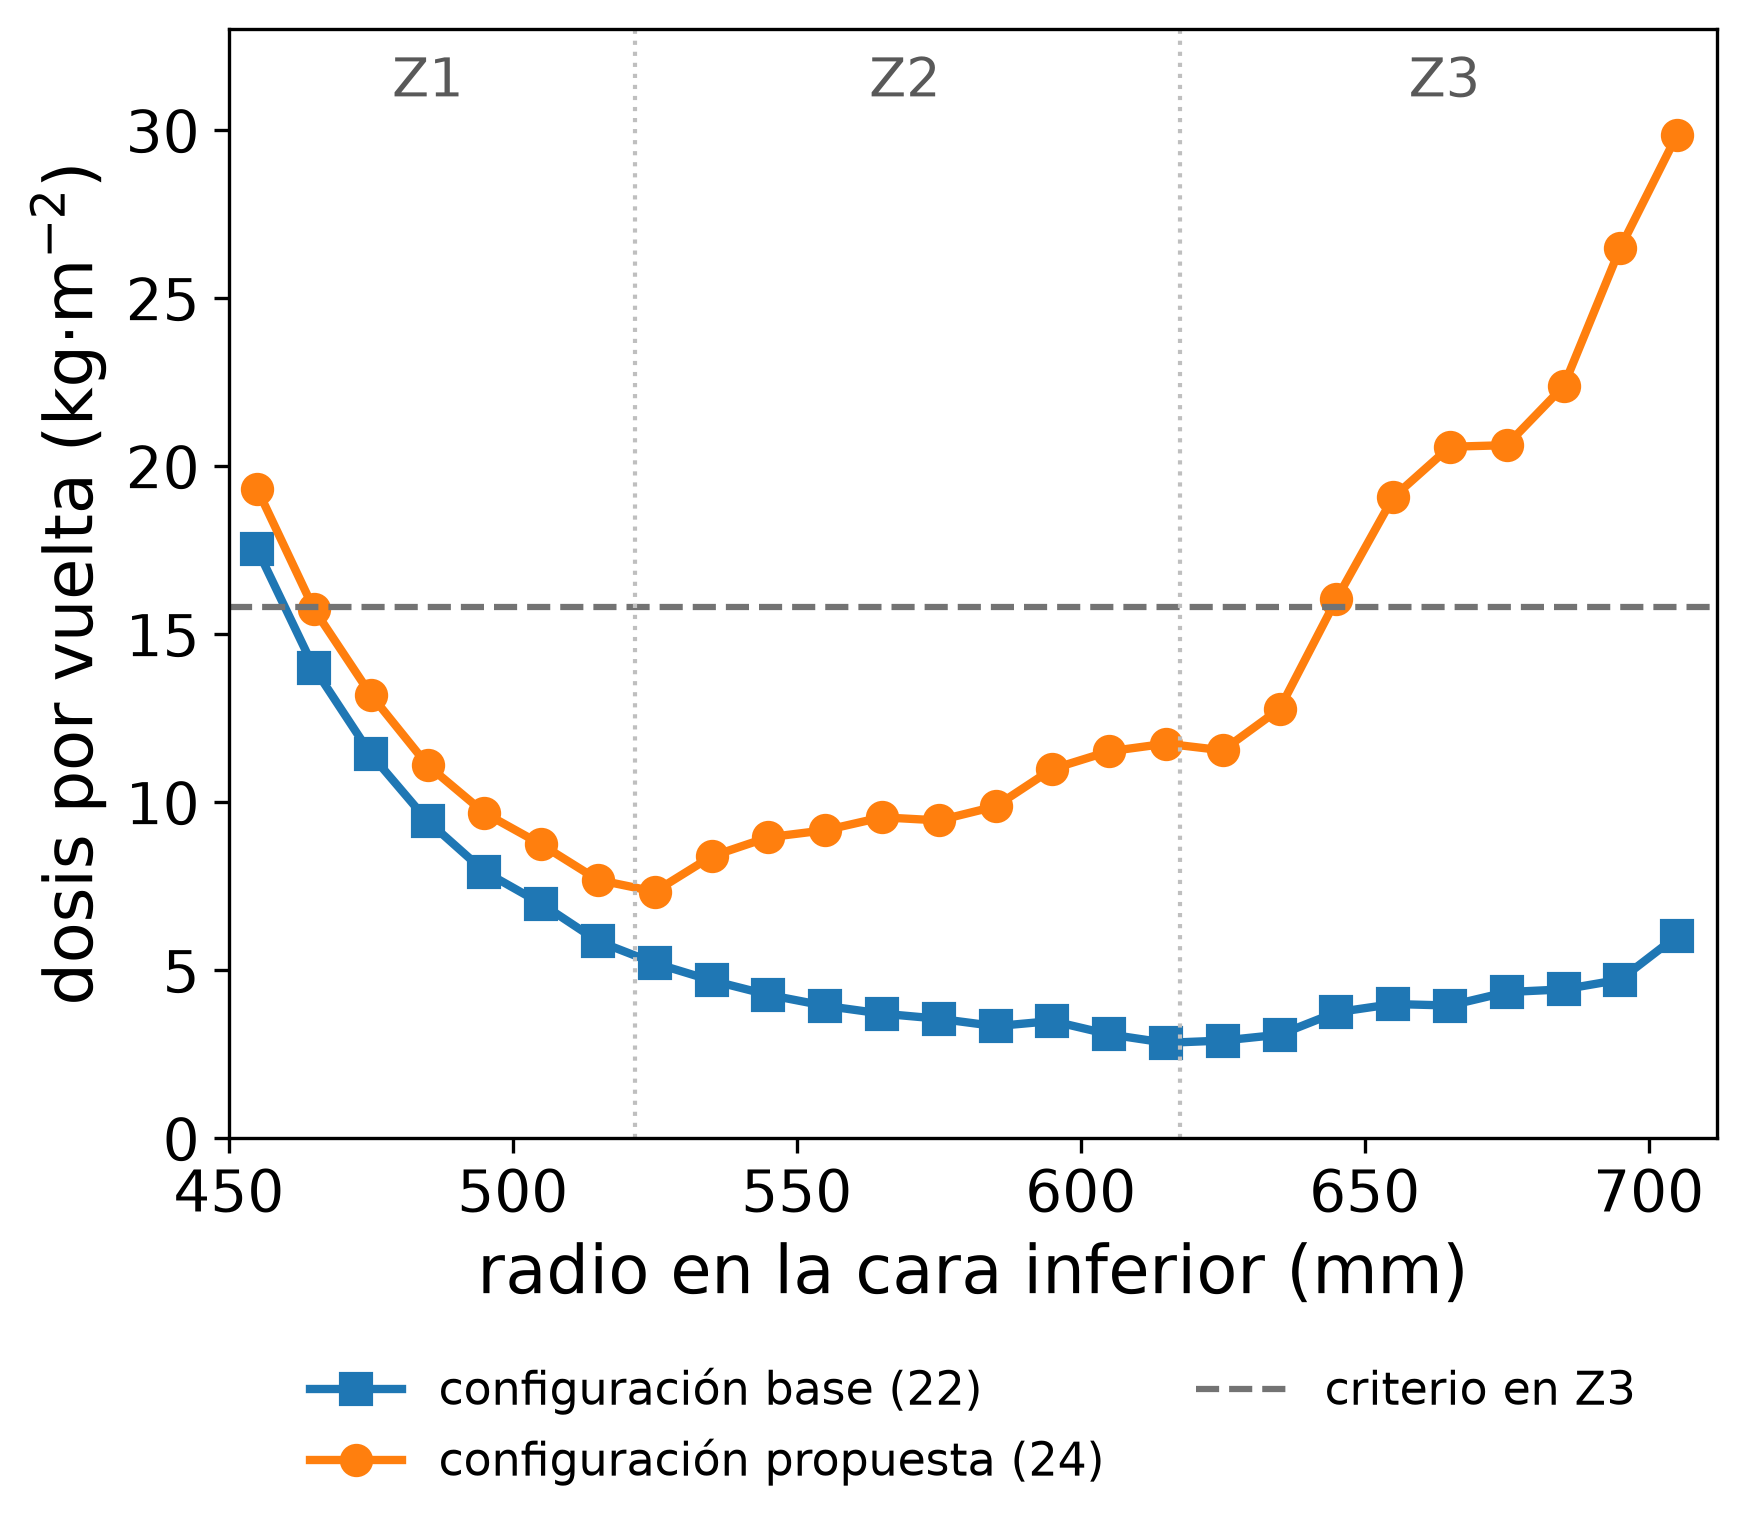
\includegraphics[width=\linewidth]{fig_dosis_cara_inferior.png}\par\small (a)
\end{minipage}\hfill
\begin{minipage}[t]{0.49\textwidth}\centering
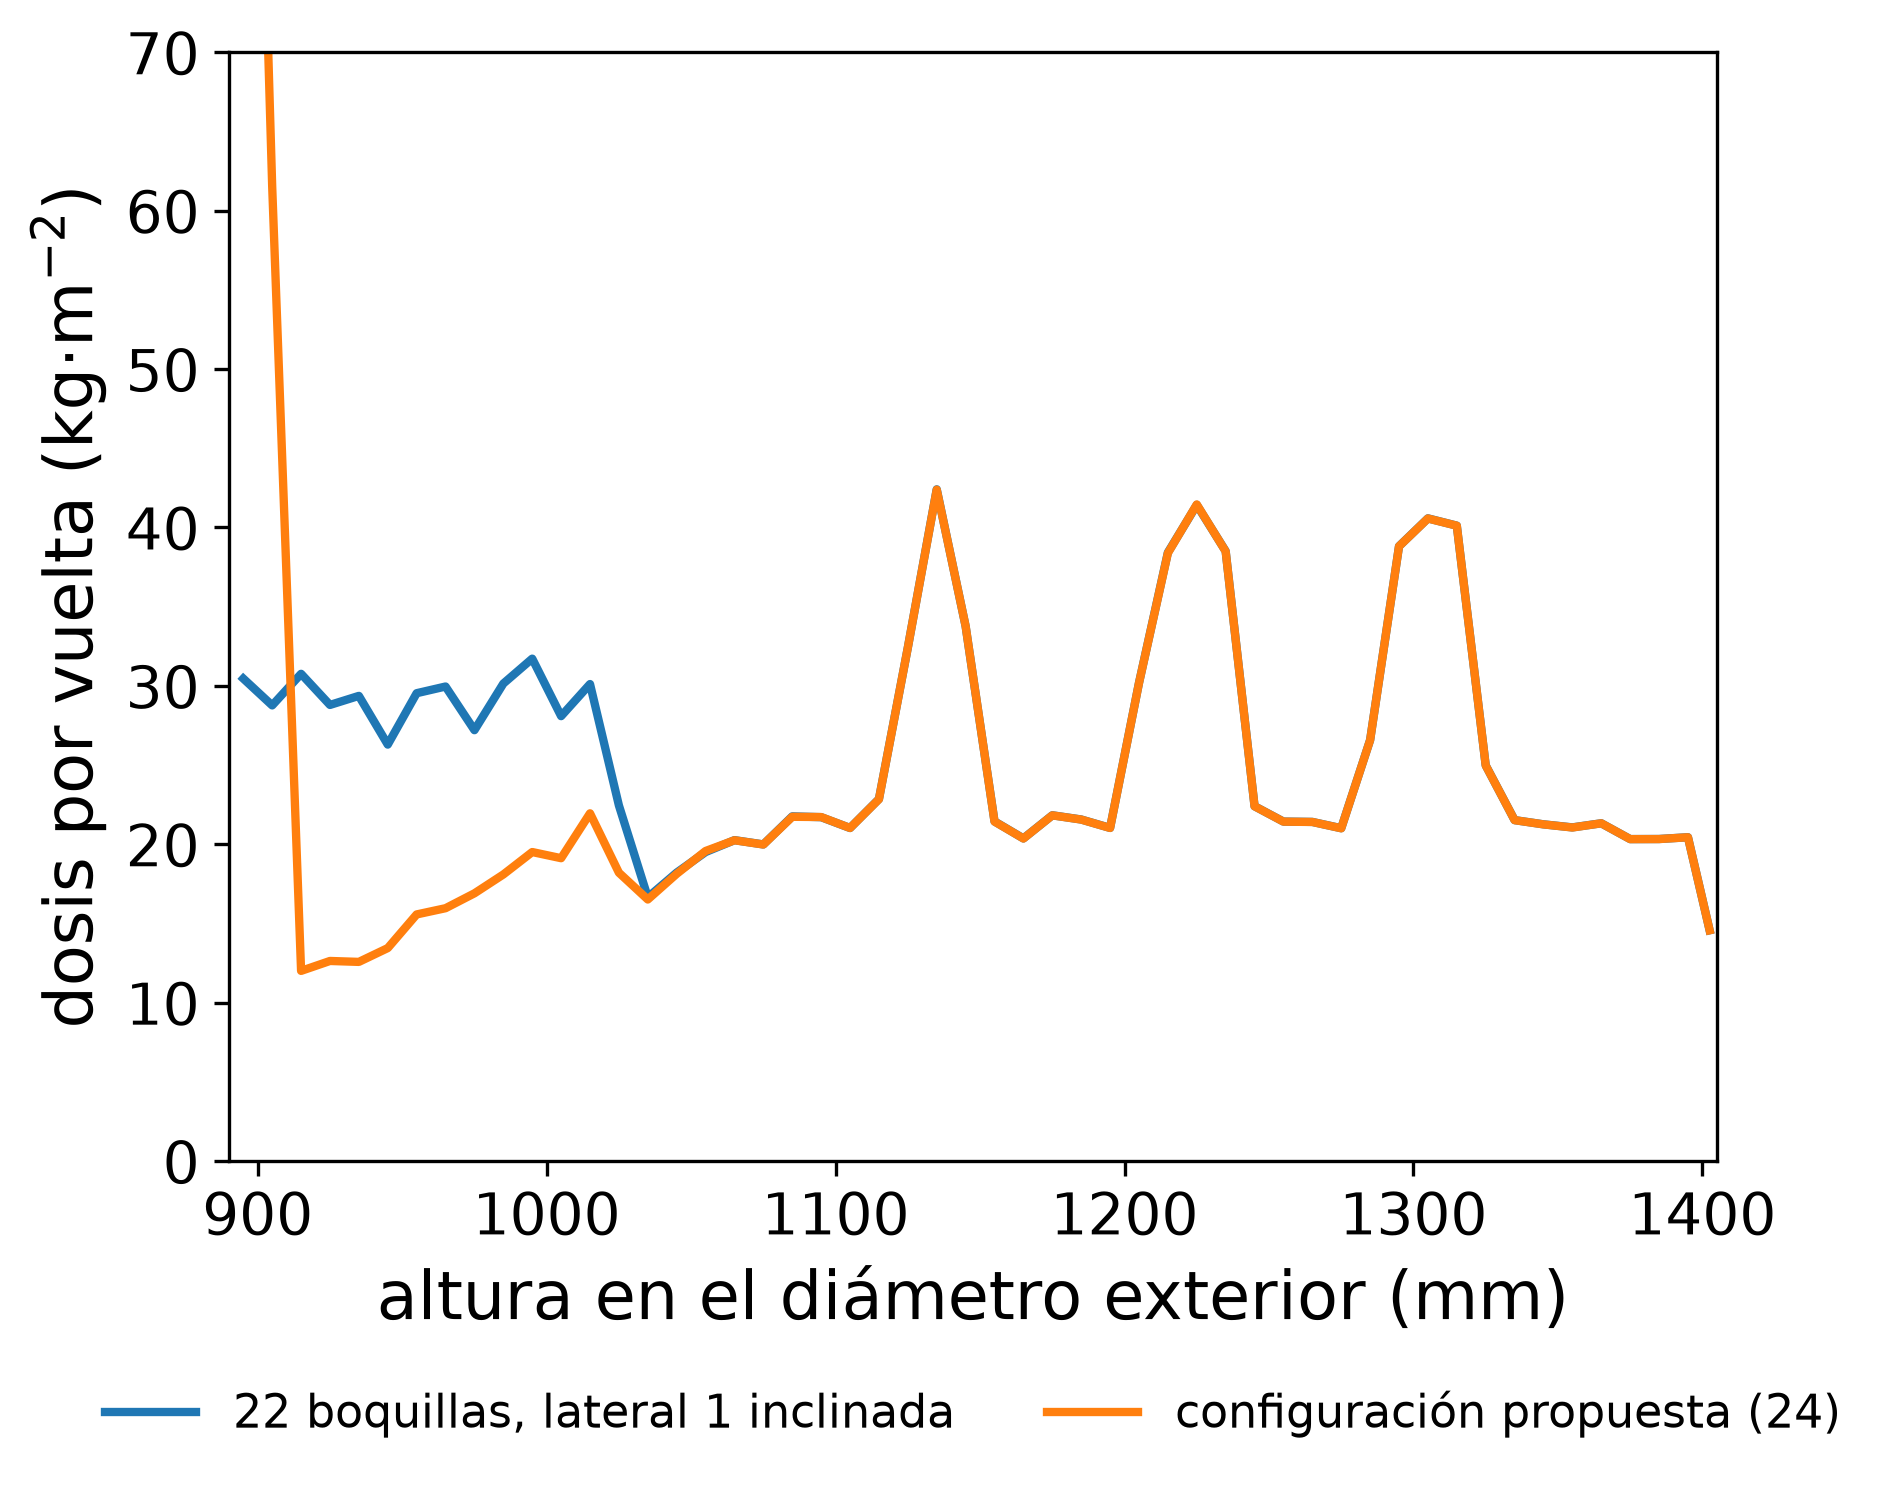
\includegraphics[width=\linewidth]{fig_dosis_diametro_exterior.png}\par\small (b)
\end{minipage}
\caption{Dosis por vuelta en bandas de 10 mm, con obstáculos: (a) cara inferior según el radio, con sus zonas Z1 (aro interior), Z2 (entre aros) y Z3 (aro exterior); (b) diámetro exterior según la altura. Elaboración propia con los datos exportados de ANSYS Fluent.}
\label{fig:cfd-propuesta}
\end{figure}

El par de boquillas inferiores cumple el criterio en la zona exterior de la cara inferior, con 19,99 frente a 15,8 kg\,m$^{-2}$ por vuelta y un coeficiente de variación de 0,298 frente a 0,4. La relación de dosis entre el diámetro exterior y la cara inferior baja de 4,8 a 1,8, y el tiempo de lavado de la cara inferior, medido en su peor banda, pasa de 36,7 a 14,7 min. Con dosis requeridas de 65 y 305 kg\,m$^{-2}$, sería de 5,2 y 24,5 min. Con ese criterio, la cara superior, cuya boquilla desplazada no se incorporó, necesita 17,6 min y es la que fija el tiempo de la máquina. Como la meta se cumplió, la reserva de elevar 25 mm los apoyos no hizo falta. El trazado de rayos había anticipado bien el resultado: esperaba de 19,6 a 19,7 en la zona exterior y el CFD dio 20,0, un 1,4\,\% más.

El cambio tiene un costo en el diámetro exterior. Las boquillas nuevas concentran agua en su borde inferior, con hasta 124 kg\,m$^{-2}$ por vuelta, y entre las alturas de 910 y 1000 mm la dosis baja de unos 29 a entre 12 y 20 (Figura~\ref{fig:cfd-propuesta}b). Frente a la configuración con la lateral inclinada, el coeficiente de variación del diámetro exterior sube de 0,265 a 0,648 y su dosis mínima baja de 14,56 a 10,53. La superficie sigue mojada por completo. Se definió para ella un criterio propio: sin zona seca y con una dosis mínima no menor que la de la superficie que fija el tiempo. Se cumple, con 0\,\% y 10,53 frente a 6,13 de la cara superior (7,33 en la cara inferior).

La verificación numérica usó tres mallas, de 202\,616, 430\,560 y 846\,960 celdas, con el número de Courant de gota cerca de 0,339 en las tres. Las dosis medias cambiaron como máximo un 0,63\,\% entre la malla base y la fina, y un 0,42\,\% al cambiar el número de parcelas (Figura~\ref{fig:cfd-malla-propuesta}); los balances de masa quedaron entre 0,024 y 0,125\,\%. No todo cumple el 2\,\%: las dosis mínimas de la cara inferior cambiaron entre 2,2 y 2,6\,\%. El orden de convergencia observado no es estable, porque algunas secuencias oscilan.

\begin{figure}[htbp]
\centering
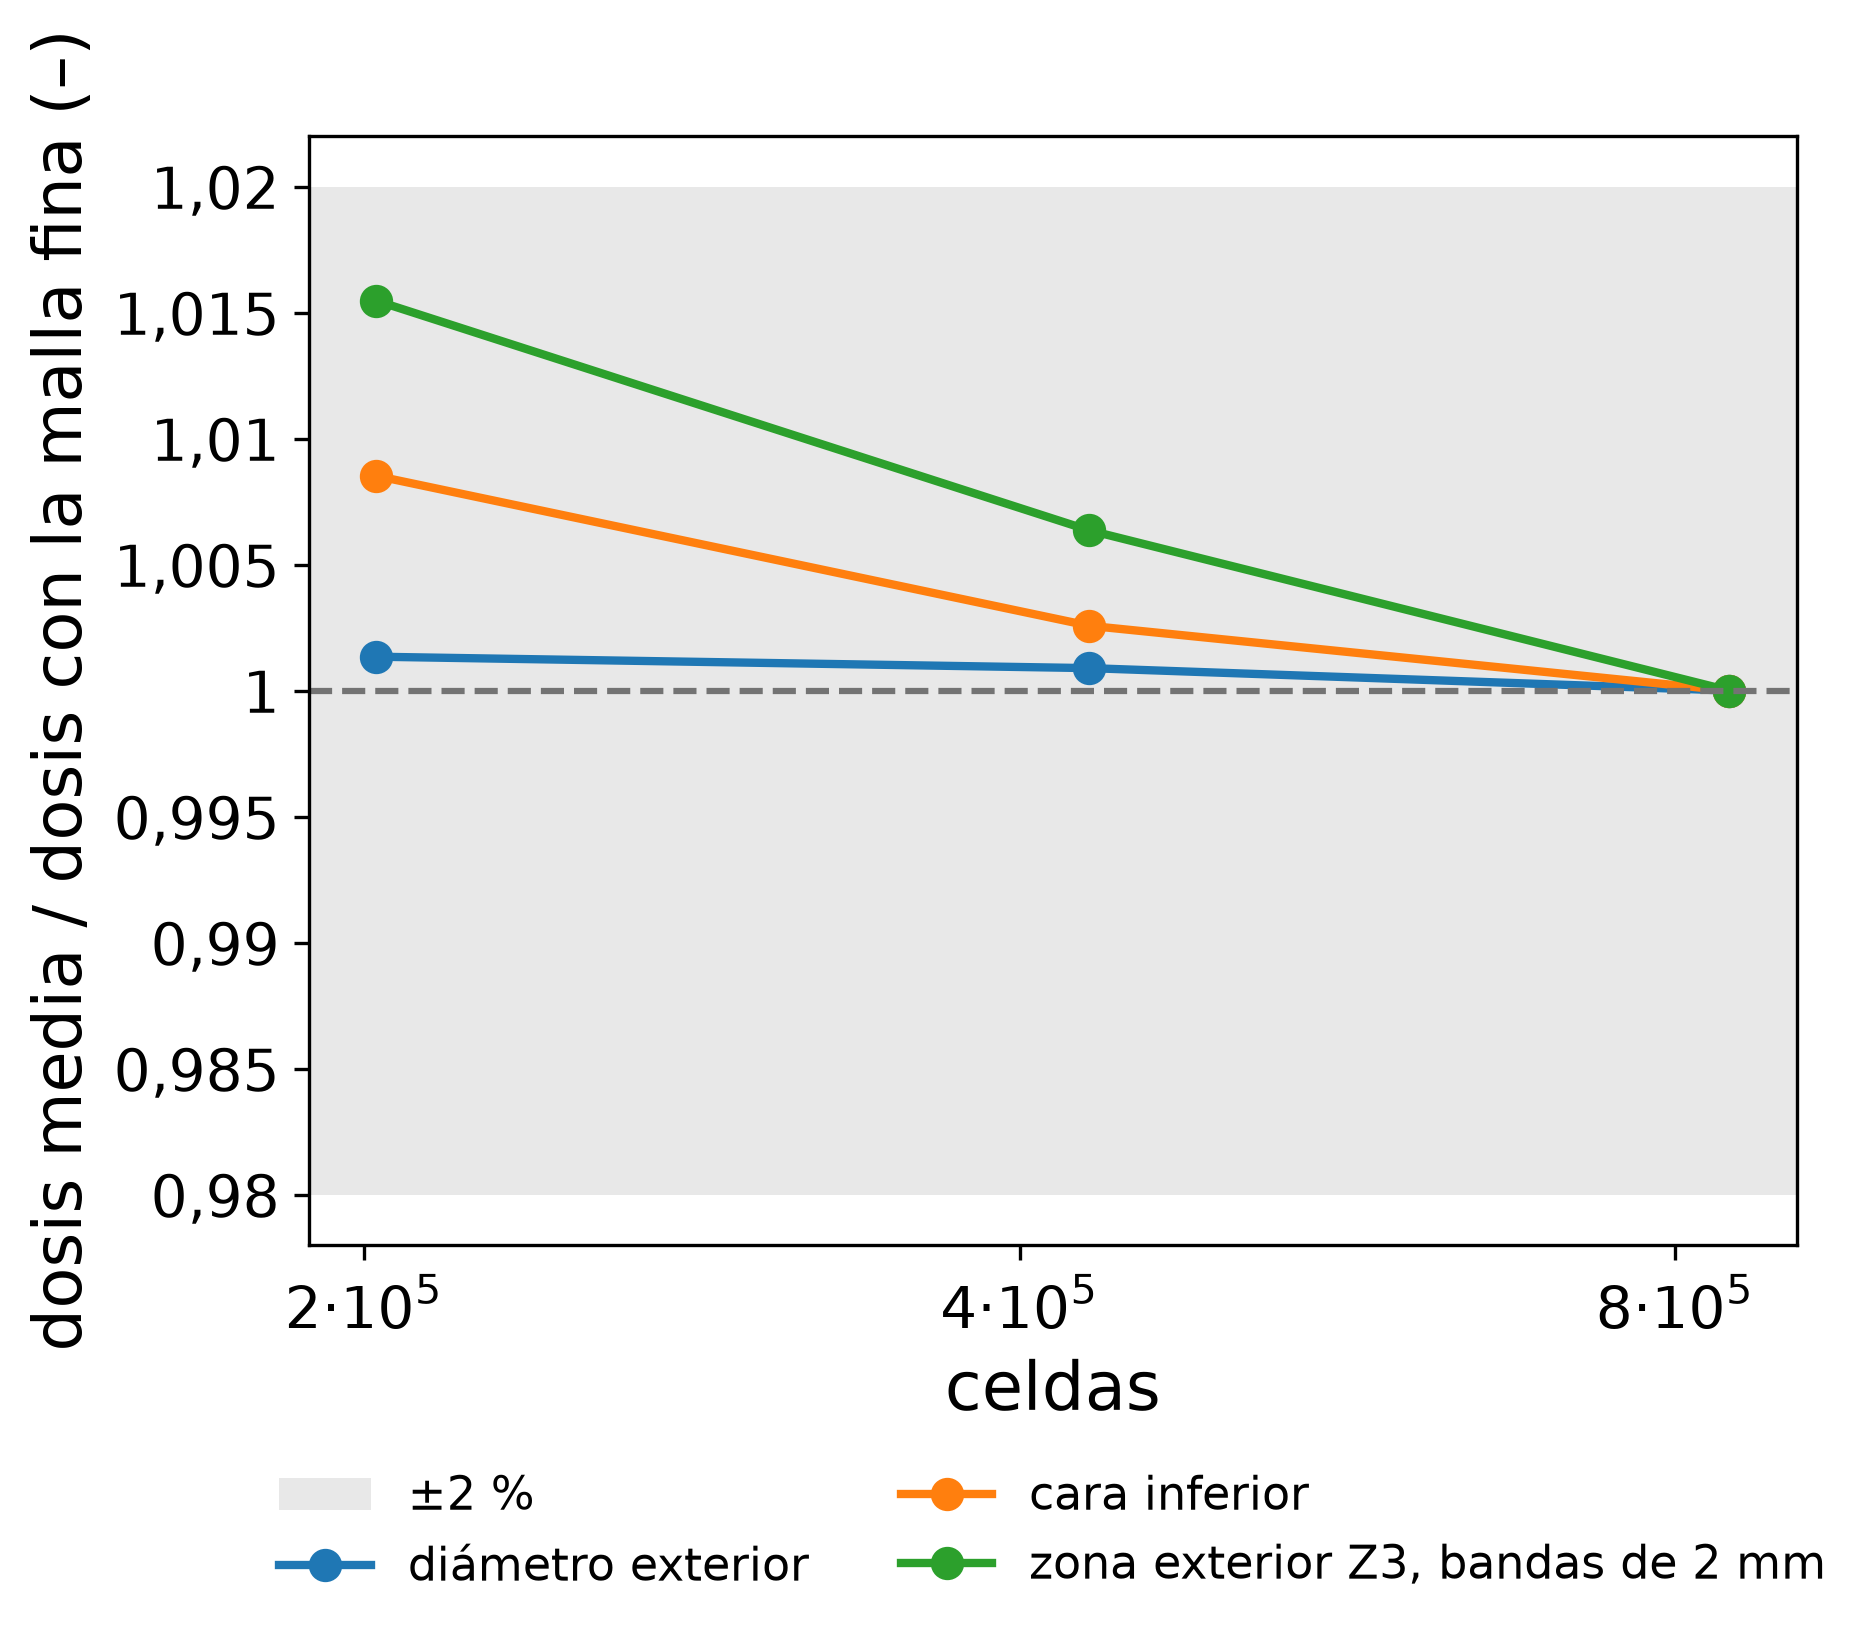
\includegraphics[width=0.55\textwidth]{fig_malla_configuracion_propuesta.png}
\caption{Dosis media de la configuración propuesta con tres mallas, normalizada con la de la malla fina. Elaboración propia con los datos exportados de ANSYS Fluent.}
\label{fig:cfd-malla-propuesta}
\end{figure}

\subsubsection{Alcance del lavado con el rodamiento armado}
\label{sec:alcance-lavado}

El lavado tiene por objetivo dejar el rodamiento en condiciones para la inspección visual inicial (Capítulo~\ref{cap:introduccion}). Su duración se estimó con el tiempo $t_{95}$ en que el 95\,\% del área accesible de cada superficie acumula una dosis requerida hipotética $D_{req}$ de 65, 183 o 305 kg\,m$^{-2}$, con la cara inferior leída por bandas de 10 mm y por celdas de 10 mm $\times$ 0,5$^\circ$, que registran las sombras parciales del soporte (Tabla~\ref{tab:tiempo-lavado}).

Con 183 kg\,m$^{-2}$, el diámetro exterior y el agujero llegan en 8,2 min y la cara superior en 10,6 min. Con el criterio del 95\,\% del área, la que más tarda es la cara inferior: con la dosis media de cada banda tarda de 5 a 24 min, pero las bases de los apoyos sectoriales y los topes dejan sombras parciales en un 14\,\% de su área, donde la dosis por vuelta es menor. Al resolver esas sombras por celdas, el tiempo sube a 27 y 76 min con 65 y 183 kg\,m$^{-2}$, y con 305 kg\,m$^{-2}$ no se alcanza en 120 min (Sección~\ref{sec:anx-tiempo-lavado}).

El lavado no alcanza el interior del rodamiento armado. Con la geometría de aros y rodillos medida en el modelo del fabricante y un trazado de rayos desde las 24 boquillas a lo largo de una vuelta del distribuidor, solo el 24\,\% del área de rodillos y pistas tiene línea de vista con alguna boquilla (Sección~\ref{sec:anx-cavidad}). La hilera inferior de rodillos queda casi oculta, con el 0,35\,\% de su superficie lateral visible, y la mitad inferior de las pistas, con el 2 al 16\,\%. Es una cota superior, porque el modelo no incluye la jaula. En ese espacio está la mayor parte de la grasa: según la regla del fabricante para el volumen libre \cite[p.~112]{skfgrasa}, el rodamiento lleno contiene de 84 a 89 kg, del mismo orden que los 75 kg de residuos por rodamiento que registra el taller (Capítulo~\ref{cap:introduccion}). El resultado cuantifica el alcance declarado: la máquina prepara las superficies exteriores para la inspección visual, y la limpieza de rodillos y pistas corresponde a la etapa con el rodamiento desarmado.

\subsection{Iteraciones de diseño}

Las iteraciones que condujeron a la configuración actual se ordenan en la Tabla~\ref{tab:iteraciones-resumen}; el registro detallado está en el Anexo~\ref{anx:iteraciones}.

\begingroup
\small\singlespacing
\setlength{\tabcolsep}{4pt}
\begin{longtable}{@{}>{\raggedright\arraybackslash}p{3.6cm}>{\raggedright\arraybackslash}p{\dimexpr(\textwidth-3.6cm-6\tabcolsep)/2\relax}>{\raggedright\arraybackslash}p{\dimexpr(\textwidth-3.6cm-6\tabcolsep)/2\relax}@{}}
\caption{Iteraciones principales del diseño}\label{tab:iteraciones-resumen}\\
\toprule
\textbf{Cambio} & \textbf{Hallazgo que lo motivó} & \textbf{Resultado}\\
\midrule\endfirsthead
\toprule
\textbf{Cambio} & \textbf{Hallazgo que lo motivó} & \textbf{Resultado}\\
\midrule\endhead
\bottomrule\endlastfoot
Mesa circular a bastidor de perfiles rectos & Muchas piezas e interfaces; ruedas en voladizo & Ruedas bajo las almas, sin ménsulas\\
Centradores de carro radial a brazo pivotante & Atravesaban los perfiles e invadían el rodamiento & Selección multicriterio: brazo pivotante\\
Uniones a momento diseñadas & La torsión de los travesaños gobernaba el centrado & Error de colocación de 3,35 mm con alas continuas\\
Límite de fuerza al empujador y ajuste H7/g6 & Error de 6,10 mm en la envolvente & 4,09 y 4,24 mm en los estados de operación\\
Rueda de 200 mm revisada & Se comparaba la carga última con la capacidad de rodadura & D/C 0,89 y 0,43; se descartó la de 250 mm\\
Empuje manual a doble cadena con volante & 325 a 837 N de empuje y 565 N de frenado & 15,5 a 39,8 N en el volante; parada con 190 N\\
Cabezal sobre monorriel a U superior giratoria con lanza & Movimiento y acceso del aplicador & Rodamiento y mesa inmóviles en el lavado\\
19 a 22 boquillas & Sin aplicación hacia la cara inferior & Acceso de 99,1\,\% por trazado de rayos\\
Lateral 1 inclinada $-4^\circ$ & Franja seca de 2 mm en el diámetro exterior & Sin zona seca\\
22 a 24 boquillas, par inferior estrecho & Cara inferior con cuatro veces menos dosis & Zona exterior de 4,1 a 20,0 kg\,m$^{-2}$ por vuelta\\
Masa del rotor medida en el CAD & La envolvente de 180 kg no cubría el rotor real & 231 kg; eje con D/C 0,27\\
Soporte superior aligerado & El criterio anterior no era funcional & De 360 a 247 kg con criterios de rigidez\\
\end{longtable}
\endgroup

\subsection{Limitaciones de los resultados}

Cada limitación que condiciona la interpretación de los resultados figura en la Tabla~\ref{tab:limitaciones-resultados} junto con la acción prevista.

\begingroup
\small\singlespacing
\setlength{\tabcolsep}{4pt}
\begin{longtable}{@{}>{\raggedright\arraybackslash}p{2.8cm}>{\raggedright\arraybackslash}p{\dimexpr(\textwidth-2.8cm-6\tabcolsep)*58/100\relax}>{\raggedright\arraybackslash}p{\dimexpr(\textwidth-2.8cm-6\tabcolsep)*42/100\relax}@{}}
\caption{Limitaciones de los resultados y acciones previstas}\label{tab:limitaciones-resultados}\\
\toprule
\textbf{Resultado} & \textbf{Limitación y efecto} & \textbf{Acción}\\
\midrule\endfirsthead
\caption[]{Limitaciones de los resultados y acciones previstas (continuación)}\\
\toprule
\textbf{Resultado} & \textbf{Limitación y efecto} & \textbf{Acción}\\
\midrule\endhead
\midrule\multicolumn{3}{r}{\textit{Continúa en la página siguiente.}}\\\endfoot
\bottomrule\endlastfoot
Análisis estructural & Apoyos bilaterales; el desvío lateral se aplicó entero a una sola rueda, lo que es conservador & Modelo con apoyo unilateral\\
Uniones y centrado & Continuidad perfecta de alas supuesta; partidas de tolerancia sin medición; disparo del limitador sin calibrar & Medición de referencias, juegos y fuerza del limitador\\
Red hidráulica & Coeficientes de pérdida estimados; altura de 53,39 o 51,0--51,3 m según el trazado; curva de la bomba leída del gráfico & Curva del fabricante y medición de presión por boquilla\\
Modelo de mojado & Retención en el primer impacto: dosis y transferencia son cotas superiores; inyección y 1,7 rpm supuestas; rodamiento con el extremo menor del agujero hacia abajo; la boquilla inferior adicional envía del 16 al 17\,\% de su caudal hacia el agujero, y que el agujero no cambie es una hipótesis & Sensibilidad a la inyección y a la orientación; corrida del agujero con la configuración propuesta\\
Limpieza & No se calcula la remoción; el VOF acota el cortante en la pared entre 5 Pa y 2 kPa (Sección~\ref{sec:anx-vof}); la dosis requerida es una hipótesis & Ensayos de huella y de remoción\\
Interior del rodamiento & 24\,\% de rodillos y pistas visible, sin la jaula & Limpieza con el rodamiento desarmado\\
Distribuidor y soporte & Tiro de la correa, carga accidental y presión supuestos; bases tomadas como empotradas & Selección de catálogo y detalle de las bases\\
Sismo & Revisión estática; la viga bajo los topes puede fluir localmente en un sismo severo & Modelo local por elementos finitos\\
\end{longtable}
\endgroup

\section{Verificación del cumplimiento de las especificaciones técnicas}
\label{sec:verificacion-especificaciones}

La Tabla~\ref{tab:cumplimiento-especificaciones} contrasta las especificaciones E01--E15 de la Tabla~\ref{tab:especificaciones_revision} con los resultados. «Cumple en el modelo» indica que el resultado numérico satisface el criterio dentro de las hipótesis del modelo.

\begingroup
\small\singlespacing
\setlength{\tabcolsep}{3pt}
\renewcommand{\arraystretch}{1.08}
\begin{longtable}{@{}p{0.75cm}>{\raggedright\arraybackslash}p{3.1cm}>{\raggedright\arraybackslash}p{4.9cm}>{\raggedright\arraybackslash}p{\dimexpr\textwidth-8.75cm-8\tabcolsep\relax}@{}}
\caption{Matriz de cumplimiento de especificaciones}\label{tab:cumplimiento-especificaciones}\\
\toprule
\textbf{Cód.} & \textbf{Criterio} & \textbf{Resultado} & \textbf{Estado}\\
\midrule\endfirsthead
\caption[]{Matriz de cumplimiento de especificaciones (continuación)}\\
\toprule
\textbf{Cód.} & \textbf{Criterio} & \textbf{Resultado} & \textbf{Estado}\\
\midrule\endhead
\midrule\multicolumn{4}{r}{\textit{Continúa en la página siguiente.}}\\\endfoot
\bottomrule\endlastfoot
E01 & Admitir 1420/900/515 mm & Envolvente en el CAD sin interferencias; paso por la puerta modelada & Cumple en el modelo; maniobra de planta pendiente\\
E02 & 3032 kg y pesos separados & 29,84 kN en los apoyos sectoriales; masa móvil de 3440 kg frente a 3500 kg de diseño & Cumple\\
E03 & Flecha $\leq L/800$ & 1,236 mm frente a 2,33 mm (también $<L/1000$) & Cumple en el nodo evaluado\\
E04 & D/C $\leq1$ & Barras del bastidor 0,82; uniones 0,58; distribuidor 0,93; soporte superior 0,18 & Cumple en el modelo\\
E05 & Reacciones compresivas sin amarre & Apoyos sectoriales y ruedas con reacciones no negativas; los pedestales del riel se anclan para $-3{,}78$ kN & Cumple en cálculo; losa por confirmar\\
E06 & Error de colocación $\leq5$ mm & 4,09 y 4,24 mm con alabeo libre; 3,35 mm con alas continuas; envolvente de 2,08 kN: 3,91 mm con alas continuas & Cumple con la fuerza final limitada a 1,95 kN\\
E07 & Carga exterior y mesa inmovilizada & Recorrido de 3320 mm; pasador con ajuste H7/g6 en carga y lavado; cadena entre estaciones & Cumple en diseño; enclavamiento en el Capítulo~\ref{cap:seguridad-ambiente}\\
E08 & Captura $\geq5$ mm & 13,1 mm en el peor caso; carrera base de 6,6 mm & Cumple numéricamente\\
E09 & 4--6 bar en la boquilla & 4,00--4,13 bar & Cumple en el modelo\\
E10 & $\leq8$ bar & Máximo de 4,13 bar & Cumple en el modelo\\
E11 & 1--3 m/s en la impulsión & 2,57 m/s en DN40 (cálculo); 1,56 m/s en DN50 (trazado) & Cumple en el modelo\\
E12 & 1--2 rpm; 30--60 s por vuelta & 1,7 rpm; 35,3 s & Valor de diseño; no medido\\
E13 & Cobertura $\geq80$\,\% (objetivo 95\,\%) & Acceso de 99,13\,\%; sin zona seca en bandas de 10 mm, ni en bandas de 2 mm del diámetro exterior con 24 boquillas & Cumple en el modelo\\
E14 & Drenaje $\geq250$ L/min & Captación de 333--350 L/min con 50\,\% de obstrucción; línea por gravedad de 413 L/min & Cumple en cálculo\\
E15 & Holgura positiva mesa--distribuidor & 18,8 mm nominal; barrido del traslado sin choques & Cumple en el CAD nominal\\
\end{longtable}
\endgroup

De las quince especificaciones, catorce se satisfacen en los modelos y en los cálculos; la velocidad del distribuidor es un valor de diseño que no se puede verificar sin el equipo. La precisión de centrado, que no se cumplía en la segunda entrega, se cumple ahora porque se limitó la fuerza del empujador y se dio continuidad a las alas del bastidor. Ninguna especificación se verificó con ensayos.

\section{Verificación del cumplimiento de restricciones}
\label{sec:verificacion-restricciones}

La Tabla~\ref{tab:cumplimiento-restricciones} verifica la configuración frente a las restricciones RS-01--RS-12 del Capítulo~\ref{cap:marco-referencial}. «Condicionada» indica que la restricción se satisface en el diseño, pero su comprobación depende de datos externos o de la implementación.

\begingroup
\small\singlespacing
\setlength{\tabcolsep}{3.5pt}
\renewcommand{\arraystretch}{1.08}
\begin{longtable}{@{}p{1.1cm}>{\raggedright\arraybackslash}p{2.6cm}>{\raggedright\arraybackslash}p{\dimexpr\textwidth-1.1cm-2.6cm-4.0cm-8\tabcolsep\relax}>{\raggedright\arraybackslash}p{4.0cm}@{}}
\caption{Verificación de restricciones}\label{tab:cumplimiento-restricciones}\\
\toprule
\textbf{Cód.} & \textbf{Restricción} & \textbf{Comprobación} & \textbf{Resultado}\\
\midrule\endfirsthead
\caption[]{Verificación de restricciones (continuación)}\\
\toprule
\textbf{Cód.} & \textbf{Restricción} & \textbf{Comprobación} & \textbf{Resultado}\\
\midrule\endhead
\midrule\multicolumn{4}{r}{\textit{Continúa en la página siguiente.}}\\\endfoot
\bottomrule\endlastfoot
RS-01 & Seguridad laboral & Secuencia que separa izaje, centrado, traslado y aspersión; traslado sin empuje directo; enclavamientos definidos (Capítulo~\ref{cap:seguridad-ambiente}) & Pasa en diseño; implementación pendiente\\
RS-02 & Técnica: masa y geometría & E01 y E02 & Pasa\\
RS-03 & Preservación & Contacto solo en superficies autorizadas; presión media de 0,85 MPa en los apoyos; presión máxima de 4,13 bar en las boquillas & Pasa en el modelo; revestimiento por confirmar con el fabricante\\
RS-04 & Espacial & Recorrido y paso por la puerta modelados & Condicionada al levantamiento del taller\\
RS-05 & Infraestructura & Pedestales anclados para levantamiento, guiado y tensor de las cadenas, con losa supuesta de 200 mm & Condicionada a la losa real\\
RS-06 & Geográfica y ambiental & Escenario de 2335 m para presión atmosférica y NPSH; zona sísmica supuesta & Condicionada a la ficha del emplazamiento\\
RS-07 & Servicios & Bomba de 4 kW, resistencias de 36 kW y circuito recirculado de 221 L/min & Pendiente de datos del taller\\
RS-08 & Ambiental y legal & Contención en cabina, pozo de drenaje y contenedor de 1000 L para la purga & Parcial; destino del efluente por definir\\
RS-09 & Química y ocupacional & Agua con detergente alcalino de baja espuma, compatible con acero y latón \cite{zep36342} & Pasa en diseño\\
RS-10 & Económica y constructiva & Presupuesto de clase 4 de S/~319\,095 sin IGV (Capítulo~\ref{cap:cronograma-presupuesto}) & No evaluable como filtro: no hay techo acreditado\\
RS-11 & Organizacional y ergonómica & Fuerza de 15,5 a 39,8 N en el volante, frente a 325--837 N de empuje directo & Pasa en cálculo; evaluación ergonómica con fuerzas medidas pendiente \cite{iso11228}\\
RS-12 & Propiedad industrial & Revisión de antecedentes conservada & Pendiente de evaluación de libertad de operación\\
\end{longtable}
\endgroup

La configuración no incumple ninguna restricción identificada, pero solo la técnica pasa sin condiciones. Las demás dependen de datos del taller, de la implementación de los controles o de ensayos. El sistema de soporte y el de aspersión quedan definidos como candidatos verificados por simulación y cálculo, no validados experimentalmente.
